\section{Versuch 14: Chat-Session}
	\develnote{�bertragung durch die Luft und mit dem Terminal-Programm die Funktion testen}

\subsection{Konzept}

Es soll eine bidirektionale Verbindung zwischen 2 entfernten PCs mit Hilfe des SPATES hergestellt werden. Das SPATES arbeitet als MODEM\footnote{MODEM: Modulator/Demodulator} und Zugriffpunkt auf den physikalischen �bertragungskanal. Da ein akustischer Kanal wie im Praktikumsraum mit den vielen auftretenden Reflexionen und St�rungen sich negativ auf die Kanalkapazit�t auswirkt, k�nnen keine hohen Daten�bertragungsraten erwartet werden.

\subsection{VHDL: Beschreibung der Hardware}

Hat das vorherige Experiment gut funktioniert, k�nnen wir durch einfache Anpassung der Frequenzen von Sender und Empf�nger die Ver�nderungen am Quellcode abschlie�en und erneut implementieren. Auch eine Simulation d�rfte hier �berfl�ssig sein.

\subsection{TEST: Praxis}

Verbinden Sie zun�chst Ihr SPATES �ber gekreuzte Signalwege, jeweils Eingang auf Ausgang, mit dem SPATES der Nachbargruppe �ber die Line-In- und Line-Out-Buchsen. 

\prohibit{Bitte nicht die Speaker- oder MIC-Buchsen verwenden, da sonst der Eingang zerst�rt werden k�nnte!}

\paragraph{Aufgabe 1}
Starten Sie nun eine Terminal-Session mit Ihrer Nachbargruppe und beobachten Sie, ob bei der �bertragung Fehler auftreten.

\paragraph{Aufgabe 2}
Verbinden Sie nun den Lausprecher mit dem SPATES und testen Sie die �bertragung durch die Luft. Beobachten Sie auch hier die H�ufigkeit von Fehlern.

\paragraph{Aufgabe 3}
Erh�hen Sie nun schrittweise die �bertragungsgeschwindigkeit in den Ter\-mi\-nal-Einstellungen Daf�r sind folgende Schritte auf beiden PCs n�tig:

\develnote{evtl. noch ein paar Icons einf�gen}

\begin{enumerate}
	\item Verbindung beenden 
\includegraphics{Part14_Chat/conclose.eps}
	\item Eigenschaften 
\includegraphics{Part14_Chat/conproperties.eps}
	\item Konfigurieren der seriellen Schnittstelle s. Abb. \ref{fig:conconfig}
	\item �betragungsgeschwindigkeit einstellen s. Abb. \ref{fig:baudrate}
	\item Die Dialoge verlassen und Verbindung herstellen 
\includegraphics{Part14_Chat/conopen.eps}
\end{enumerate}

\begin{figure}[ht]
	\centering
	\begin{minipage}[c]{.41\linewidth}
		\centering
			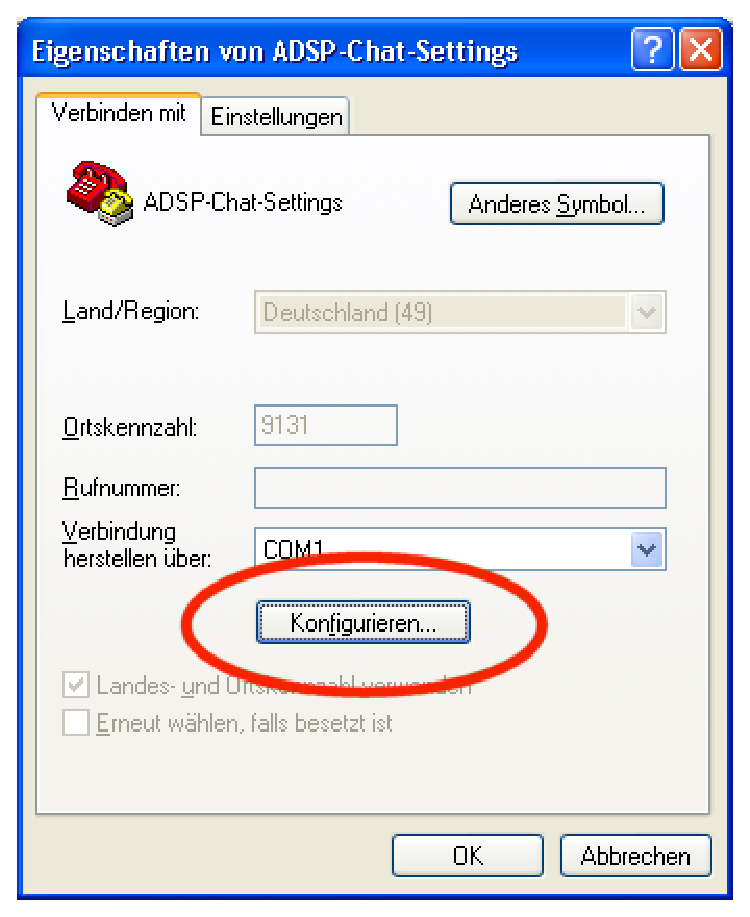
\includegraphics[height=18em]{Part14_Chat/conconfig.eps}
		\caption{HyperTerm-Eigenschaften}
		\label{fig:conconfig}
	\end{minipage}
	\begin{minipage}[c]{.10\linewidth}
		\hfill
	\end{minipage}
	\begin{minipage}[c]{.41\linewidth}
		\centering
			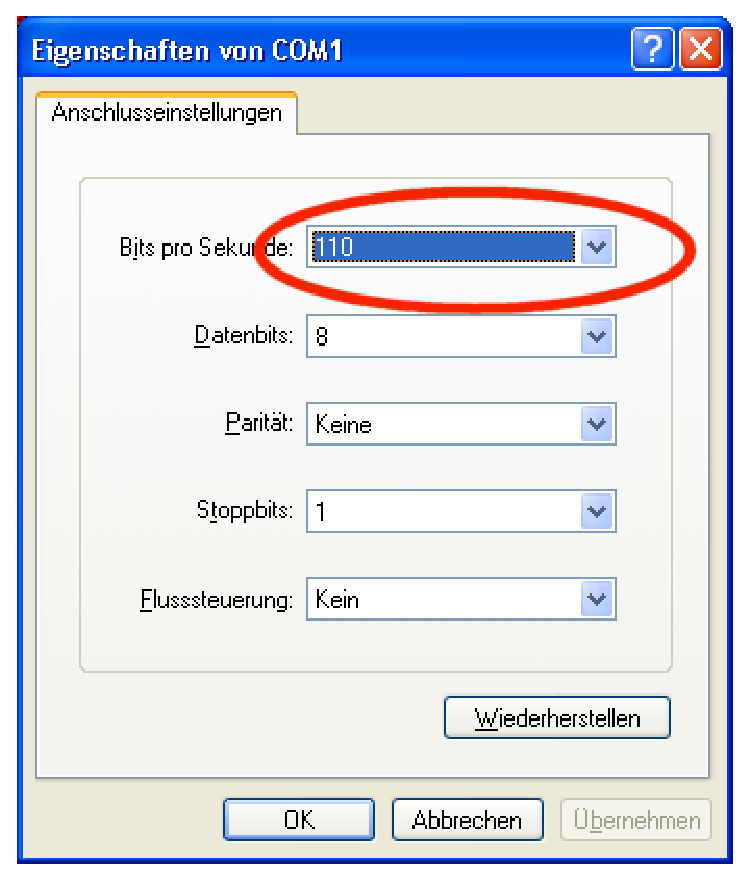
\includegraphics[height=18em]{Part14_Chat/baudrate}
		\caption{Einstellen der �bertragungsrate}
		\label{fig:baudrate}
	\end{minipage}
\end{figure}

Bis zu welcher maximalen �bertragungsgeschwindigkeit ist eine Daten�bertragung mit tolerierbarer Fehlerrate m�glich? Welche 4 Modulationsfrequenzen Frequenzen wurden bei Ihnen zugeteil?

\answergame{3}{Tja, das kommt ganz drauf an}

Welche einfachen �nderungen k�nnen Sie durchf�hren, um die �bertragungsgeschwindigkeit zu steigern?

\answergame{3}{Erh�hen der Modulationsfrequenzen}

Welche grundlegenden �nderungen w�ren n�tig, um im gleichen Frequenzbereich und der gleichen �bertagungsstrecke wesentlich h�here �bertragungsraten zu realisieren?

\answergame{3}{Anderes Modulationsverfahren, Fehlerkorrektur-Mechanismen,...}

Sollte noch etwas Zeit sein, k�nnen sie versuchen, eine gemeinsame Modulationsfrequenz f�r alle SPATES zu verwenden.